\documentclass[12pt,a4paper,bibliography=totocnumbered,listof=totocnumbered]{scrartcl}
\usepackage[ngerman]{babel}
\usepackage[utf8]{inputenc}
\usepackage{amsmath}
\usepackage{amsfonts}
\usepackage{amssymb}
\usepackage{graphicx}
\usepackage{fancyhdr}
\usepackage{tabularx}
\usepackage{geometry}
\usepackage{setspace}
\usepackage[right]{eurosym}
\usepackage[printonlyused]{acronym}
\usepackage{subfig}
\usepackage{floatflt}
\usepackage[usenames,dvipsnames]{color}
\usepackage{colortbl}
\usepackage{paralist}
\usepackage{array}
\usepackage{titlesec}
\usepackage{parskip}
\usepackage{acronym}
\usepackage[modulo]{lineno}
\pagewiselinenumbers
\usepackage{footmisc}
\usepackage[right]{eurosym}
\usepackage[subfigure,titles]{tocloft}
\usepackage[pdfpagelabels=true]{hyperref}
\usepackage{comment}

\usepackage{listings}
\lstset{basicstyle=\footnotesize, captionpos=b, breaklines=true, showstringspaces=false, tabsize=2, frame=lines, numbers=left, numberstyle=\tiny, xleftmargin=2em, framexleftmargin=2em}
\makeatletter
\def\l@lstlisting#1#2{\@dottedtocline{1}{0em}{1em}{\hspace{1,5em} Lst. #1}{#2}}
\makeatother

\geometry{a4paper, top=27mm, left=30mm, right=20mm, bottom=35mm, headsep=10mm, footskip=12mm}

\hypersetup{unicode=false, pdftoolbar=true, pdfmenubar=true, pdffitwindow=false, pdfstartview={FitH},
	pdftitle={Bachelorarbeit},
	pdfauthor={Fabian Wilms},
	pdfsubject={Bachelorarbeit},
	pdfcreator={\LaTeX\ with package \flqq hyperref\frqq},
	pdfproducer={pdfTeX \the\pdftexversion.\pdftexrevision},
	pdfkeywords={Bachelorarbeit},
	pdfnewwindow=true,
	colorlinks=true,linkcolor=black,citecolor=black,filecolor=magenta,urlcolor=black}
\pdfinfo{/CreationDate (D:20110620133321)}

\begin{document}

\titlespacing{\section}{0pt}{12pt plus 4pt minus 2pt}{-6pt plus 2pt minus 2pt}

% Kopf- und Fusszeile
\renewcommand{\sectionmark}[1]{\markright{#1}}
\renewcommand{\leftmark}{\rightmark}
\pagestyle{fancy}
\lhead{}
\chead{}
\rhead{\thesection\space\contentsname}
\lfoot{Generative Testerstellung für Microservice-Architekturen}
\cfoot{}
\rfoot{Seite \thepage}
\renewcommand{\headrulewidth}{0.4pt}
\renewcommand{\footrulewidth}{0.4pt}

% Vorspann
\renewcommand{\thesection}{\Roman{section}}
\renewcommand{\theHsection}{\Roman{section}}
\pagenumbering{Roman}

% ----------------------------------------------------------------------------------------------------------
% Titelseite
% ----------------------------------------------------------------------------------------------------------
\thispagestyle{empty}
\begin{center}
	
\includegraphics[scale=0.25]{images/Hochschule_Muenchen_Logo.png}\\
	\vspace*{2cm}
	\Large
	\textbf{Fakultät für Informatik und Mathematik 07}\\
	\vspace*{2cm}
	\Huge
	\textbf{Bacheloararbeit}\\
	\vspace*{0.5cm}
	\large
	über das Thema\\
	\vspace*{1cm}
	\textbf{Generative Testerstellung für Microservice-Architekturenit}\\
	\vspace*{2cm}
	
	\vfill
	\normalsize
	\newcolumntype{x}[1]{>{\raggedleft\arraybackslash\hspace{0pt}}p{#1}}
	\begin{tabular}{x{6cm}p{7.5cm}}
		\rule{0mm}{5ex}\textbf{Autor:} & Fabian Wilms\newline holtkoet@hm.edu \\ 
		\rule{0mm}{5ex}\textbf{Prüfer:} & Prof. Dr. Ulrike Hammerschall \\ 
		\rule{0mm}{5ex}\textbf{Abgabedatum:} & xx.xx.2017 \\ 
	\end{tabular} 
\end{center}
\pagebreak

% ----------------------------------------------------------------------------------------------------------
% Abstract
% ----------------------------------------------------------------------------------------------------------
\setcounter{page}{1}
\onehalfspacing
\titlespacing{\section}{0pt}{12pt plus 4pt minus 2pt}{2pt plus 2pt minus 2pt}
\rhead{KURZFASSUNG}
\section{Kurzfassung}

kurzfassung

\vspace{-1,2em}
\titlespacing{\section}{0pt}{12pt plus 4pt minus 2pt}{-6pt plus 2pt minus 2pt}
\section*{Abstract}

Das ganze auf Englisch.

\pagebreak

% ----------------------------------------------------------------------------------------------------------
% Verzeichnisse
% ----------------------------------------------------------------------------------------------------------
% TODO Typ vor Nummer
\renewcommand{\cfttabpresnum}{Tab. }
\renewcommand{\cftfigpresnum}{Abb. }
\settowidth{\cfttabnumwidth}{Abb. 10\quad}
\settowidth{\cftfignumwidth}{Abb. 10\quad}

\titlespacing{\section}{0pt}{12pt plus 4pt minus 2pt}{2pt plus 2pt minus 2pt}
\singlespacing
\rhead{INHALTSVERZEICHNIS}
\renewcommand{\contentsname}{II Inhaltsverzeichnis}
\phantomsection
\addcontentsline{toc}{section}{\texorpdfstring{II \hspace{0.35em}Inhaltsverzeichnis}{Inhaltsverzeichnis}}
\addtocounter{section}{1}
\tableofcontents
%\pagebreak
\rhead{VERZEICHNISSE}
\listoffigures
%\pagebreak
\listoftables
%\pagebreak
\renewcommand{\lstlistlistingname}{Listing-Verzeichnis}
{\labelsep2cm\lstlistoflistings}
%\pagebreak

% ----------------------------------------------------------------------------------------------------------
% Abkürzungen
% ----------------------------------------------------------------------------------------------------------
\section{Abkürzungsverzeichnis}
\begin{acronym}[DDD] % längste Abkürzung steht in eckigen Klammern
	\acro{DDD}{Domain-Driven Design}
	\acro{LHM}{Landeshauptstadt München}
\end{acronym}
\newpage

% ----------------------------------------------------------------------------------------------------------
% Inhalt
% ----------------------------------------------------------------------------------------------------------
% Abstände Überschrift
\titlespacing{\section}{0pt}{12pt plus 4pt minus 2pt}{-6pt plus 2pt minus 2pt}
\titlespacing{\subsection}{0pt}{12pt plus 4pt minus 2pt}{-6pt plus 2pt minus 2pt}
\titlespacing{\subsubsection}{0pt}{12pt plus 4pt minus 2pt}{-6pt plus 2pt minus 2pt}

% Kopfzeile
\renewcommand{\sectionmark}[1]{\markright{#1}}
\renewcommand{\subsectionmark}[1]{}
\renewcommand{\subsubsectionmark}[1]{}
\lhead{Kapitel \thesection}
\rhead{\rightmark}

\onehalfspacing
\renewcommand{\thesection}{\arabic{section}}
\renewcommand{\theHsection}{\arabic{section}}
\setcounter{section}{0}
\pagenumbering{arabic}
\setcounter{page}{1}
\setcounter{secnumdepth}{6}

% ----------------------------------------------------------------------------------------------------------
% Einführung und Motivation
% ----------------------------------------------------------------------------------------------------------
\section{Einführung und Motivation}

IT nimmt sowohl im privaten als auch geschäftlichen Alltag eine immer größere Rolle ein. Die Übernahme von Bereichen, die ehemals als nicht durch Computer austauschbar erachtet wurden, schreitet immer weiter fort. Doch dadurch steigen nicht nur bestehende Anforderungen an Software, sondern es entstehen auch neue Kriterien. Ganz abgesehen davon steigt die Komplexität von modernen Software-Systemen immens an.

Mit steigender Komplexität und höherer Nachfrage am Markt, sowie engen Zeitplänen für Projekte wird leider häufig aus Zeit- und Kostengründen auf Qualität nur geringfügig Rücksicht genommen. Zunächst verursacht eine gute Software-Qualität nämlich nur Mehrkosten. Personelle wie zeitliche. Die langfristige Sinnhaftigkeit bleibt dabei außen vor, aus der Vergangenheit wird nur selten gelernt.

Ein Bericht der Kölner Beratungsfirma SQS zeigt anhand von gesammelten Zahlen aus Beratungsaufträgen welche immensen Kosten durch unentdeckte Fehler entstehen. Hier wird besonders deutlich wie viel es für ein Projekt bedeutet, frühzeitige Qualitätssicherung durchzusetzen. Und dazu zählt auch das Testen von Software.

\vspace{1em}
\begin{minipage}{\linewidth}
	\centering
	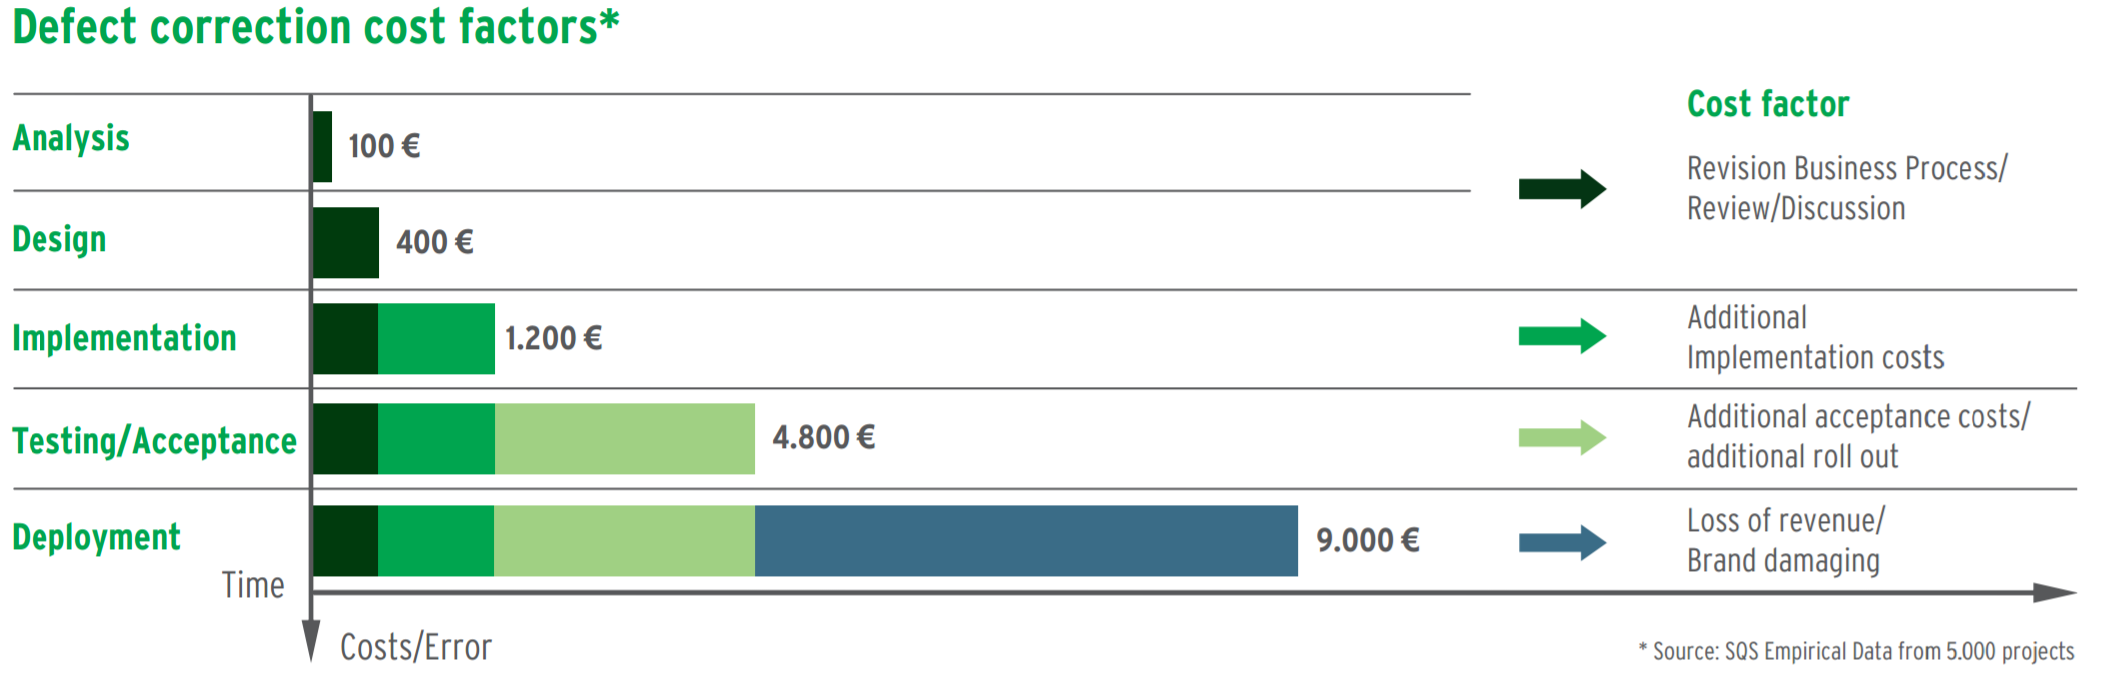
\includegraphics[width=0.9\linewidth]{images/img_sqs-defect-correction.PNG}
	\captionof{figure}[SQS Report Costs of Defect Correction]{SQS Report Costs of Defect Correction \cite{sqsdefect}}
	\label{fig:img_sqs-defect-correction}
\end{minipage}

Umso früher Fehler entdeckt und bemerkt werden, umso weniger kostet es auch diese zu beheben. Wenn bereits vor dem Start der Implementierungsphase auf eine hohe Testabdeckung, beispielsweise durch den Einsatz von test-driven development, wert gelegt wird, können, je auftretendem Fehler, um die 7800\euro\\cite{sqsdefect} eingespart werden. Mit diesen Zahlen sind die Mehrkosten, die für ein solches vorgehen entstehen um ein vielfaches leichter zu rechtfertigen.

Somit sorgt das Bug-Fixing in Produktivsystemen, also das Beheben sogenannter \textit{field defects}, für einen der größten Kostenfaktoren. Wurde in den ersten Phasen eines Projekts nicht viel, oder kein Wert auf eine ausreichende Test-Abdeckung gelegt schaffen es viele Fehler in die Produktivsysteme der Hersteller. Doch werden diese Fehler erst im laufenden Betrieb beim Kunden festgestellt, ist es bereits zu spät. Robert N. Charette kritisiert eben dies in seinem Artikel \textit{Why Software Fails}\cite{charette}.

\begin{quote}
	\begin{itshape}
		If the software coders don't catch their omission until final system testing--or worse, until after the system has been rolled out--the costs incurred to correct the error will likely be many times greater than if they'd caught the mistake while they were still working on the initial [...] process.
	\end{itshape}
\end{quote}

Die Lösung sollte also sein, viel Zeit und Geld in gute Softwarequalität zu investieren. Jedoch stehen, wie bereits am Anfang der Einleitung erwähnt, Projektleiter und ihre Mitarbeiter unter hohem zeitlichen Druck. Und Testen kostet neben Geld auch Zeit. Es entsteht in dieser Zeit aber kein Fortschritt an der Funktionalität der Software. Dies ist auch der Grund, weshalb das Testen bei Entwicklern nicht an oberster Stelle der liebsten Aufgaben steht. Es kostet Zeit ohne erkennbaren Fortschritt zu erreichen.

Bei it@M, dem Eigenbetrieb der Landeshauptstadt München, ist eine hohe Testabdeckung daher Teil der Definition of Done [citation needed] von Softwareprojekten. Im Kommunalen Umfeld sind die zeitlichen Restriktionen noch einmal stärker zu gewichten als in der freien Wirtschaft. Viele Projekte werden aufgrund von anstehenden Gesetzesänderungen ins Leben gerufen und müssen mit Inkrafttreten der neuen Regelungen in Produktion gehen. it@M ist somit ständig auf der Suche nach Lösungen, die den Entwicklungs- und Testprozess beschleunigen, um die geringe Zeit möglichst effizient nutzen zu können.

Eine dieser Lösungen wurde im letzten Jahr von Martin Kurz im Rahmen seiner Masterarbeit\cite{mkthesis} geplant und entwickelt. Die Model-driven Software Development Lösung Barrakuda \footnote{Github Repository von Barrakuda (https://github.com/xdoo/mdsd)}. Diese bietet den Entwicklern von it@M die Möglichkeit anhand von einer vorgegebenen Domänen-spezifischen Sprache Microservice-Architekturen zu modellieren und diese zu generieren.

Im Rahmen dieser Arbeit soll eine Erweiterung von Barrakuda geplant und entwickelt werden. Diese Weiterentwicklung soll einen Großteil verschiedener Testmethoden für diese Architektur generieren und die benötigte Entwicklungszeit für eine hohe Testabdeckung möglichst stark reduzieren.

Zunächst wird die Microservice Architektur im generellen und anschließend im speziellen anhand der von it@M Vorgegebene Architektur genauer erläutert und die zu testenden Komponenten identifiziert.

Anschließend werden bekannte Methoden zum testen von Software analysiert und in Hinblick der Umsetzungsmöglichkeit im generativen Ansatz geprüft. Zusätzlich werden alternative Methoden, die besonders im Bereich der Microservices anzutreffen sind, ebenfalls untersucht.

Schließlich sollen Anforderungen, die an die zu generierenden Tests gestellt werden festgehalten werden, die im letzten Abschnitt, der Implementierung, Beachtung finden werden.

% ----------------------------------------------------------------------------------------------------------
% Architektur-Generierung für Software-Projekte
% ----------------------------------------------------------------------------------------------------------
\section{Architektur}

Sam Newman stellt in seinem Buch \textit{Building Microservices} einige Vorteile dar, die Microservices gegenüber Monolithischen Architekturen bieten\cite{buildingms}:

Die Heterogenität, welche es erlaubt, für verschiedene Einsatzzwecke verschiedene SPrachen und Technologien zu verwenden, ohne das ganze System damit implementieren zu müssen.

Die erhöhte Widerstandsfähigkeit gegenüber Fehlern im System, da die Grenzen von Microservices eine Kaskadierung von Fehlern verhindern können.

Microservices lassen sich leichter skalieren. Während monolithische Architekturen immer im ganzen Skaliert werden, kann man in einer Microservice-Architektur nach genau die Services skalieren, die in diesem Moment mehr Leistung benötigen.

Ein weiterer Punkt ist ein einfacheres Deployment. Insbesondere kleinen Änderungen führen bei monolithischen Systemen zu einem großen Overhead, während man in einer Microservice Architektur nur den Service neu deployen muss, der auch die implementierte Änderung enthält.

Ebenfalls lässt sich die Team-Organisation vereinfachen. Ein Team arbeitet an einem Service, dessen Funktionalität klar definiert ist, anstatt ein großes Team zu haben, wessen Teilteams an teilen eines Monolithen arbeiten.

Auch optimieren Microservices die Austauschbarkeit. Die kleinen abgegrenzten Systeme lassen sich mit viel weniger aufwand gegen neuere oder bessere Implementierungen austauschen, ohne andere Komponenten zu Gefährden. Während dies bei Monolithischen Anwendungen zu unvorhersehbaren Problemen kommen kann, weshalb in solchen Architekturen auch häufig kaum Änderungen durchgeführt werden.

Dies sind einige der Gründe, warum mit Barrakuda eine Microservice-Architektur für it@M generiert wird. Sie behandelt einen Großteil der Probleme, die bei bestehenden Systemen der Landeshauptstadt aufgetreten sind.

\subsection{Microservice Architektur und Unterschiede zur monolithischen Architektur}

Um die Vorteile dieser Architektur in einem System effektiv zu nutzen gibt es bereits in der Planung einiges zu beachten.

Dazu zählt, dass es zwei Dinge gibt, die einen guten Microservice ausmachen. Lose Kopplung und Starker Zusammenhalt \cite[S.62]{buildingms}.

Lose Kopplung bedeutet, dass Änderungen an einem Service keine Änderungen an einem anderen Service nach sich ziehen. Ist dies nicht gegeben, ist einer der Hauptvorteile von dieser Art Architektur nicht mehr vorhanden.
Ein lose gekoppelter Service weiß von seinem Kommunikationspartner nur so wenig wie möglich.\cite[S.63]{buildingms}

Starker Zusammenhalt soll dafür sorgen, dass bestimmte Funktionalitäten an einem Ort vorhanden sind, sodass diese leicht geändert werden können und nicht mehrere Komponenten angepasst werden müssen.\cite[S.64]{buildingms}

Zum Planen einer Software mit Mircoservice Architektur ist es sinnvoll, sich zunächst über Kontextgrenzen (\textit{bounded context}) Gedanken zu machen. Kontextgrenzen sind eine Definition aus dem Buch \textit{Domain Driven Design} von Eric Evans \cite{dddesign}, welches auch von Newman herangezogen wird.

Eine Kontextgrenze soll eine logische Grenze darstellen, welche über eine Schnittstelle verfügt, die festlegt, welche Informationen mit anderen Kontexten geteilt wird.\cite[S.65]{buildingms}. Damit einher geht die Unterscheidung zwischen geteilten und versteckten Modellen. Versteckte Modelle werden innerhalb einer Kontextgrenze benötigt, sind aber für andere Kontexte uninteressant. Geteilte Modelle hingegen werden über die Grenzen hinweg freigegeben. Sind solche Kontextgrenzen für eine Software modelliert, lassen sich aus diesen sehr leicht Microservices ableiten, da bereits einige Grundvoraussetzungen getroffen sind: Lose Kopplung und Starker Zusammenhalt.\cite[S.68]{buildingms}

\begin{quote}
	\begin{itshape}
		[I]f our service boundaries align to the bounded contexts in our domain, and our microservices
		represent those bounded contexts, we are off to an excellent start in ensuring that our microservices
		are loosely coupled and strongly cohesive.\cite{buildingms}
	\end{itshape}
\end{quote}

\subsubsection{Kommunikation zwischen Services}

Als weiterer Schritt muss eine Kommunikationsart zwischen Services und zur Außenwelt definiert werden.

\paragraph{Geteilte Datenbanken} werden dafür gerne verwendet. \cite[S.85]{buildingms}. Dies birgt allerdings viele Probleme. Jede noch so kleine Änderung an der "Logik" dieser Datenbank, oder an der internen Struktur der Daten muss mit viel Bedacht durchgeführt werdenm, da jede abhängige Komponente sonst nicht mehr funktionieren könnte.

Des weiteren ist die technologische Einschränkung ein großer Nachteil. Wenn auch es in den ersten Schritten der Planung und Entwicklung Sinnvoll erscheint eine relationale Datenbank zu verwenden, können spätere Geschäftsentscheidungen oder neu auftretende Probleme den Einsatz einer Graphdatenbank sinnvoller machen. Bei einer geteilten Datenbank eine solche Änderung durchzuführen ist sehr schwierig\cite[S.85]{buildingms}.

\paragraph{Remote Procedure Calls (RPCs)}\label{rpcpara} sind eine weitere bekannte Kommunikationsmöglichkeit. Ein Vorteil von RPC ist, dass es sehr einfach und schnell möglich ist Methoden der Services für Clients und andere Services Verfügbar zu machen. Über die Kommunikation muss man sich nahezu keine Gedanken machen\cite[S.91]{buildingms}.

Doch die Nachteile überwiegen schnell und deutlich. Je nach Implementierung führt die Verwendung von RPC zu einer starken Bindung an eine bestimmte Sprache (bekanntestes Beispiel Java RMI). Auch verstecken RPC-Implementierungen die Komplexität der entfernten Aufrufe. Dies kann zu starken Performance-Problemen führen, wenn Entwickler an Interfaces arbeiten, von denen sie denken es seien lokale Methoden\cite[S.93]{buildingms}.

Die Verwendung von RPC macht die Weiterentwicklung von Systemen nicht einfacher: Ein Beispiel anhand einer Schnittstelle zur Instanziierung eines Kunden. Zusätzlich zur Erstellung eines Kunden mithilfe seines Namen und einer E-Mail Adresse soll es nun eine Möglichkeit geben diesen nur mithilfe seiner Mail-Adresse zu erstellen. Das reine hinzufügen einer neuen Methode in einem Interface löst das Problem in diesem Fall nicht. Im schlimmsten Fall benötigen alle Clients die diesen Service ansprechen die neuen Stubs und müssen allesamt neu Bereitgestellt werden\cite[S.94]{buildingms}. Und das bereits bei einer so kleinen Änderung.

\paragraph{REpresentational State Transfer (REST)} ist eine der meistgenutzten Architekturstilen für APIs \cite{duvander}. REST wird, auch wenn die Spezifikation es nicht vorschreibt, in den häufigsten Fällen über HTTP genutzt \cite[S.97]{buildingms}. Dies rührt daher, dass beispielsweise die bekannten HTTP-Methoden POST, GET, PUT usw. machen es sehr einfach die geforderte homogene Verhaltensweise von Methoden auf allen Ressourcen umzusetzen. Auch wird HTTP gerne genutzt, da es bereits eine breite Masse an bestehenden Tools gibt die zur weiteren Qualitätsverbesserung eines Systems genutzt werden können, wie zum Beispiel Proxies und Load Balancer. Doch dies sind alles zunächst nur Vorteile von HTTP.

Die Verwendung von REST bietet viele Möglichkeiten die lose Kopplung zwischen Services zu ermöglichen. Dazu zählt unter anderem Hypermedia As the Engine of Application State (HATEOAS). HATEOAS ist ein Teil der REST-Spezifizierung und beschreibt ein Konzept, nach dem, einfach gesagt, Informationen Links zu anderen Informationen enthalten. Um bei dem Kundenbeispiel aus \ref{rpcpara} zu bleiben: Wird die Information eines Kunden abgerufen, kann das Kundenobjekt zusätzlich zu den Kundendaten ein Feld enthalten welches zur Bestellliste dieses Kund zeigt.

\lstinputlisting{code/customer.json}

Mit der Verwendung von HATEOAS reicht es, wenn alle Clients die Kundendaten und deren Bestellungen verarbeiten wissen, dass Kunden einen Link-Feld mit dem Typ "orders" besitzen. Wenn also später Services unter anderen Adressen erreichbar sind, oder sich interne Datenstrukturen ändern müssen diese Clients nicht neu angepasst werden.

\paragraph{JSON oder XML?} 

Wenn die Entscheidung über den Weg der Kommunikation gefallen ist muss die Art der Kommunikation festgelegt werden. JSON und XML sind dabei die größten Namen. In den vergangenen Jahren ist dabei die Verwendung von XML im Gegensatz zu JSON in APIs zurückgegangen\cite{duvander2}. Jedoch bieten beide Vor- wie Nachteile. JSON ist das einfachere Format und auch leichtgewichtiger, während XML einige sinnvolle Features wie z.B. link control (insbesondere für HATEOAS interessant) oder auch das extrahieren von Teilinformationen durch Standards wie in etwa XPATH\cite[S.101]{buildingms}.

\paragraph{Authentifizierung} todo

\paragraph{Continous Delivery} todo

Die Entscheidungen, welche Technologien und Architekturen in der von Barrakuda generierte Architektur verwendet werden sind bereits von it@M getroffen worden. Im folgenden wird die generierte Architektur kurz erläutert.


\subsection{Vorgegebene Architektur der LHM}

Die von Barrakuda generierte Microservice-Architektur verwendet das Spring-Framework. Auslöser dafür ist, dass bei it@M größtenteils Java-Entwickler arbeiten und diese bereits mit Java EE viel Erfahrung gesammelt haben. Da das Spring-Framework auf viele Konzepte von Java EE aufbaut, erleichtert dies den Einstieg in die Microservice-Welt für kommende Entwicklungen.

Die generierten Services kommunizieren über eine REST-API, die ihre Daten im JSON-Format überträgt. HATEOAS wird über Spring HATEOAS genutzt.

Als Datenbank in der Entwicklungsumgebung kommt eine In-Memory-Datenbank von H2 zum Einsatz. In der Produktion größtenteils Oracles JDBC-Datenbank in der Version 7, aber auch MySQL wird verwendet.

Zur Authentifizierung wird ein Authentifizierungs-Service generiert, der zusätzlich zur internen Nutzer- und Rechteverwaltung auch eine Anbindung an das Stadtweite LDAP bietet.

Das Problem der Entdeckbarkeit von Service wird mithilfe von Netflixs Eureka-Service gelöst. Dieser bietet innerhalb einer Domäne einen Zentralen Anlaufpunkt für alle Services um sich dort zu vermerken, sowie Informationen über die Adressen von anderen Services einzuholen.

Clients können mit der Domäne über ein API-Gateway kommunizieren (Netflix Zuul). Dieses öffnet nach außen eine einzige Schnittstelle, über die sowohl eine graphische Nutzeroberfläche aufgerufen, als auch die einzelnen Services kontaktiert werden können. Auch ermöglicht das Gateway den Zugriff auf bestimmte Endpunkte zur sperren, was für die Landeshauptstadt insbesondere für Software interessant ist, die sowohl interne, als auch externe Schnittstellen bieten soll.

Auch werden Docker-Konfigurationen mitgeliefert, um die Continous Delivery mithilfe eines Container-Frameworks zu ermöglichen.

\vspace{1em}
\begin{minipage}{\linewidth}
	\centering
	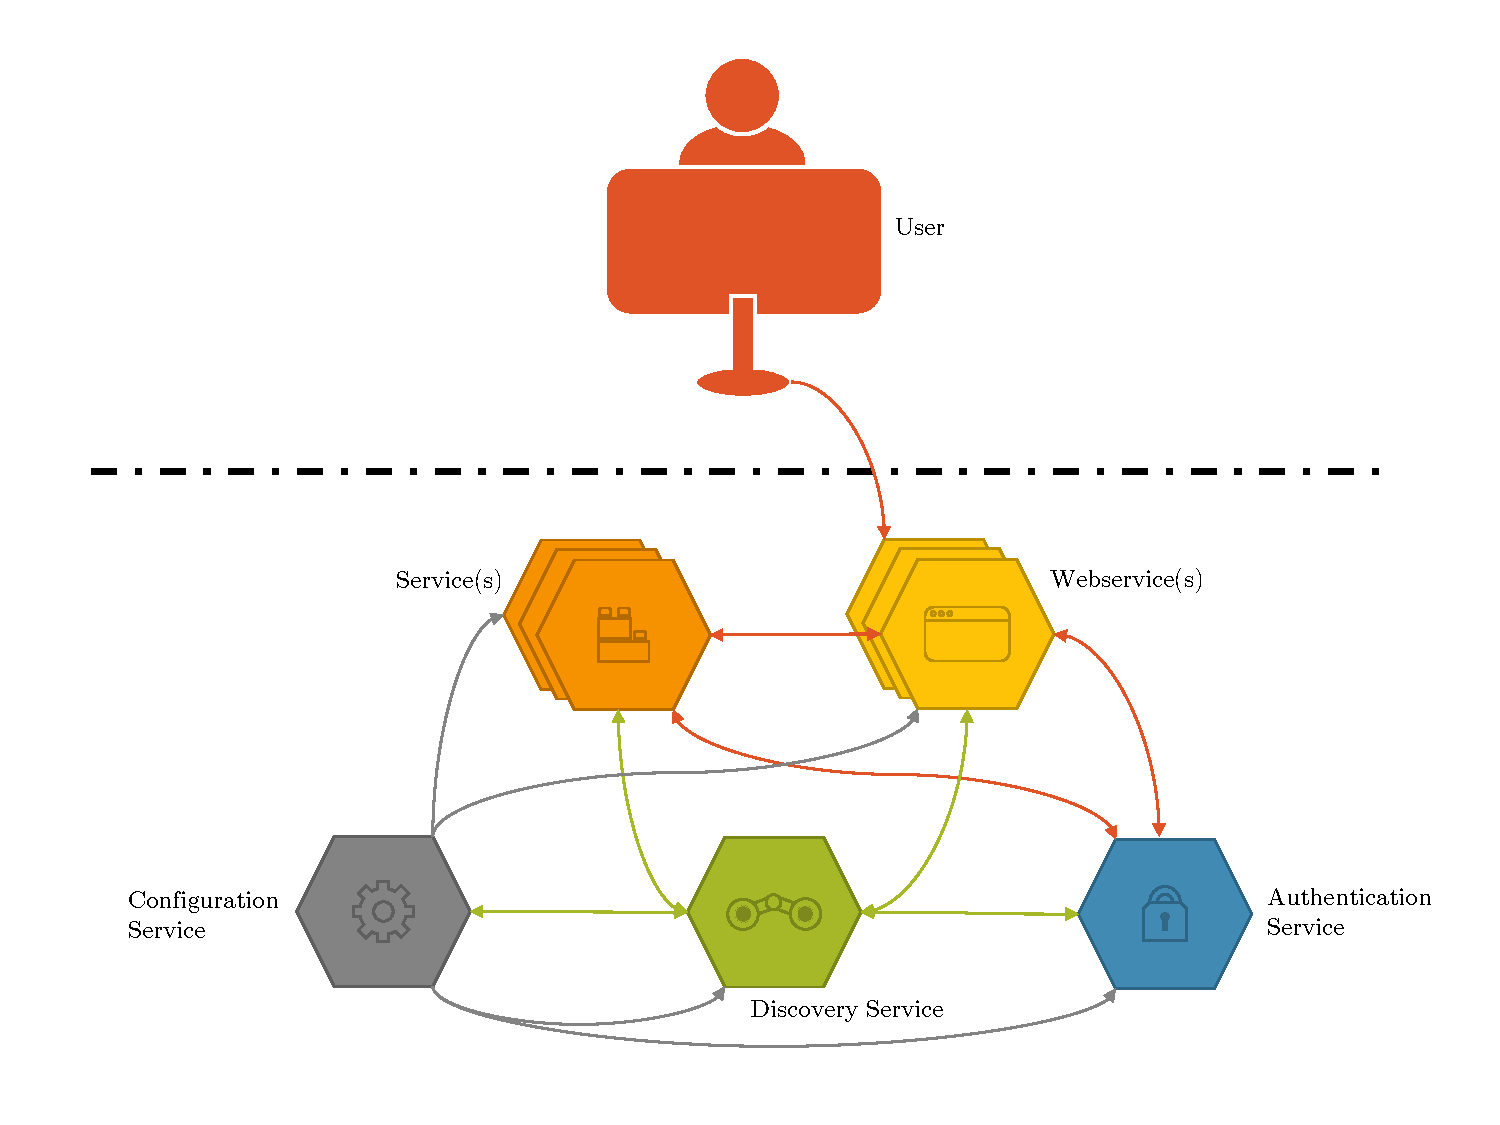
\includegraphics[width=0.9\linewidth]{images/img_arch-stadt-gesamt.pdf}
	\captionof{figure}[Architekturvorgabe it@M]{Architekturvorgabe it@M}
	\label{fig:img_arch-stadt-gesamt}
\end{minipage}

Intern sehen die generierten komponenten so aus:

\subsubsection{Authentifizierungsservice}

\subsubsection{Discoveryservice}

\subsubsection{Configurationservice}

\subsubsection{Service}

\subsubsection{Webservice}

\subsection{Unterschiede zwischen Microservices und Monolith-Architekturen}

\subsubsection{Auswirkungen}

% ----------------------------------------------------------------------------------------------------------
% Software Testen
% ----------------------------------------------------------------------------------------------------------

\section{Software Testen}

\subsection{Bekannte Testmethoden}

\begin{comment}
performance, security, usability, compatability...

\vspace{1em}
\begin{minipage}{\linewidth}
	\centering
	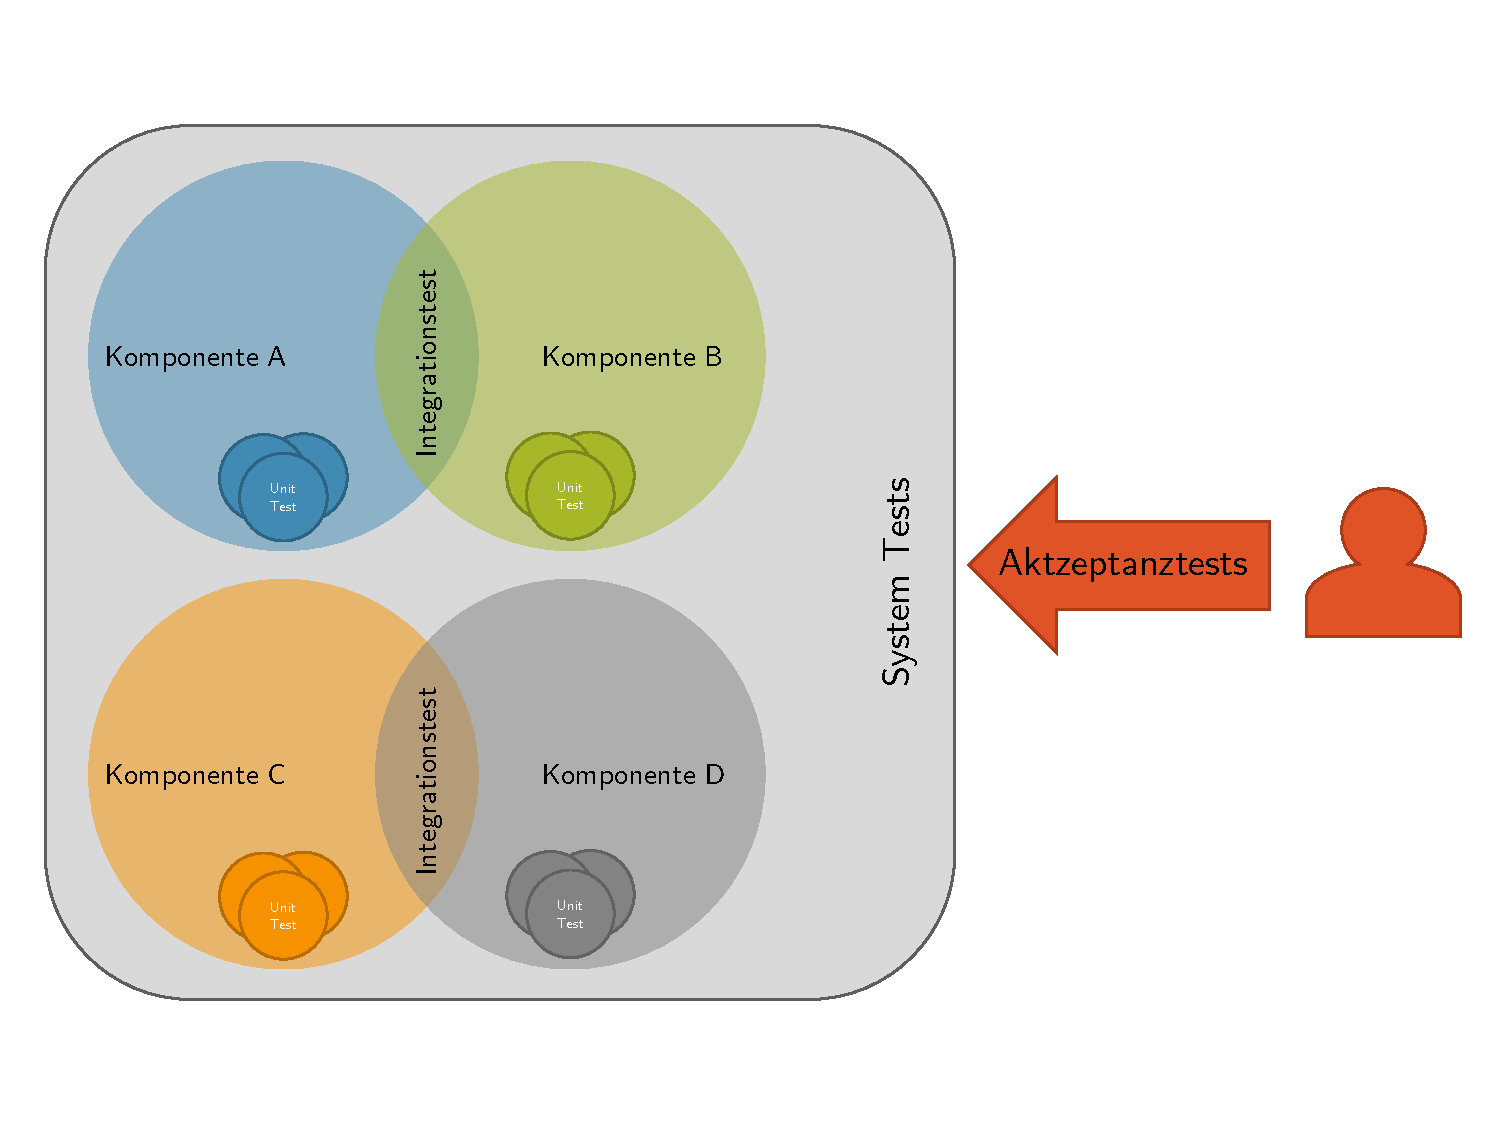
\includegraphics[width=0.9\linewidth]{images/img_testmethods_functional.pdf}
	\captionof{figure}[Bekannte Testmethoden]{Bekannte Testmethoden}
	\label{fig:img_testmethods_functional}
\end{minipage}
\end{comment}

\subsection{Testen von Microservices}

\paragraph{Unit Tests}


\begin{comment}
\vspace{1em}
\begin{minipage}{\linewidth}
	\centering
	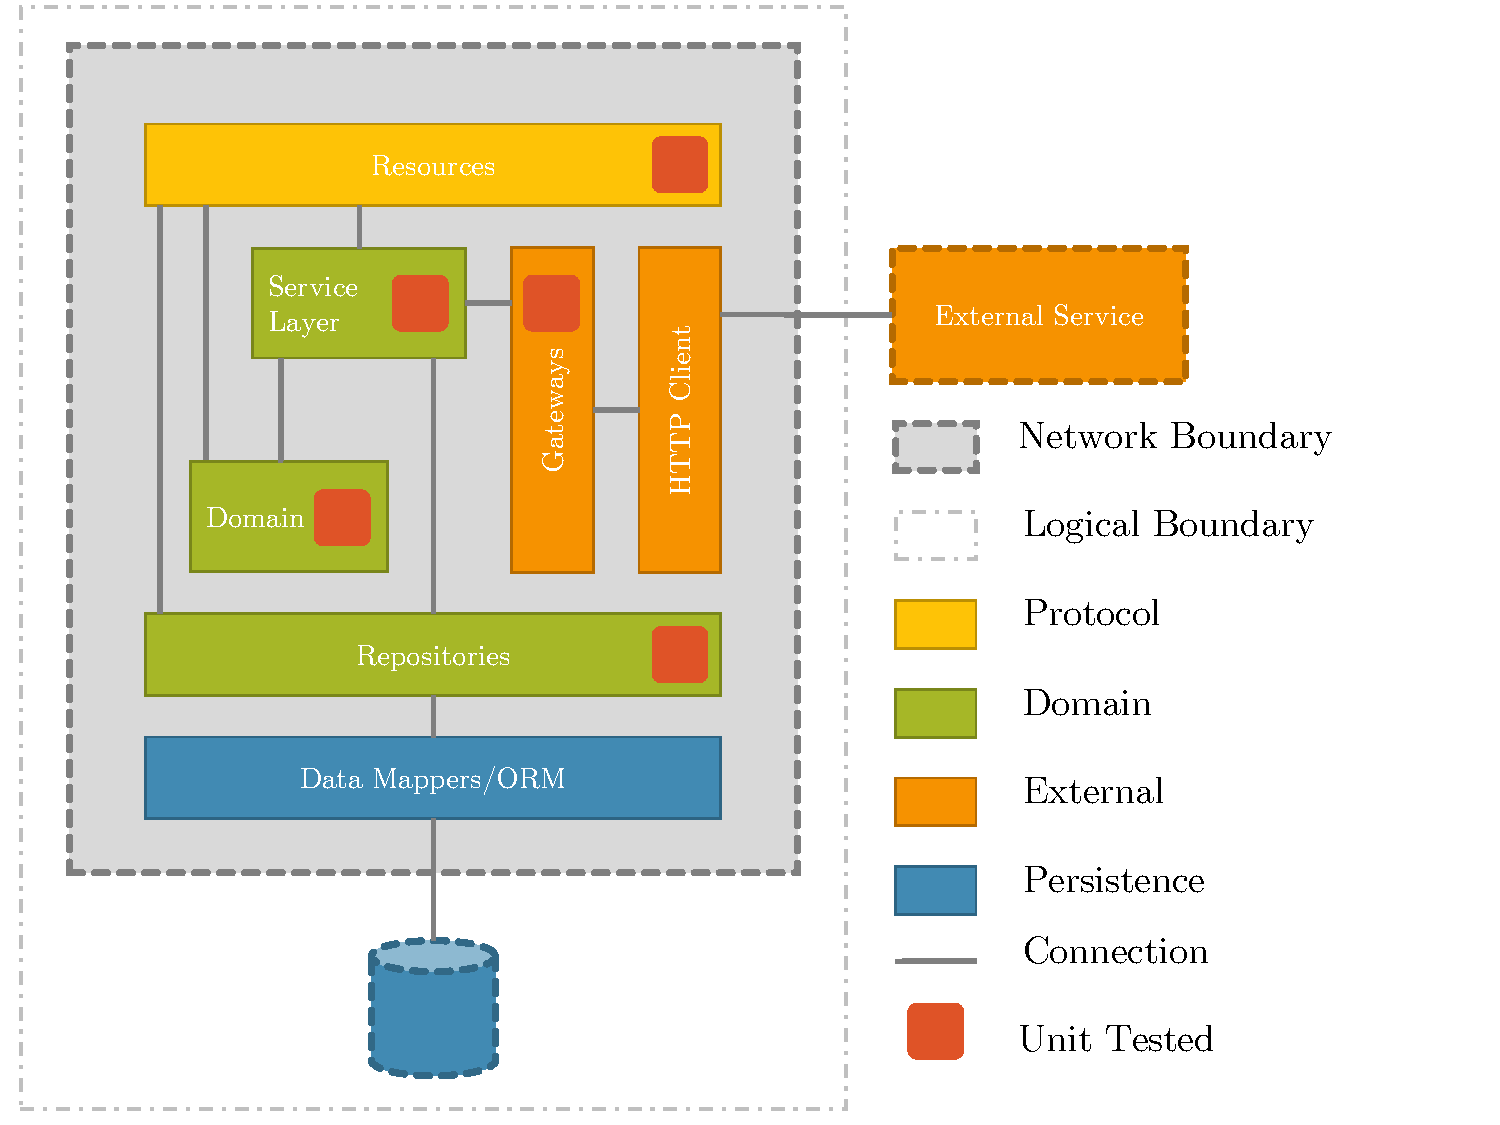
\includegraphics[width=0.9\linewidth]{images/img_unit-testing.pdf}
	\captionof{figure}[Unit Testing Scope]{Unit Testing Scope \cite{clemson}}
	\label{fig:img_unit-testing}
\end{minipage}
\end{comment}

\paragraph{Integrationstests}


\begin{comment}
\vspace{1em}
\begin{minipage}{\linewidth}
	\centering
	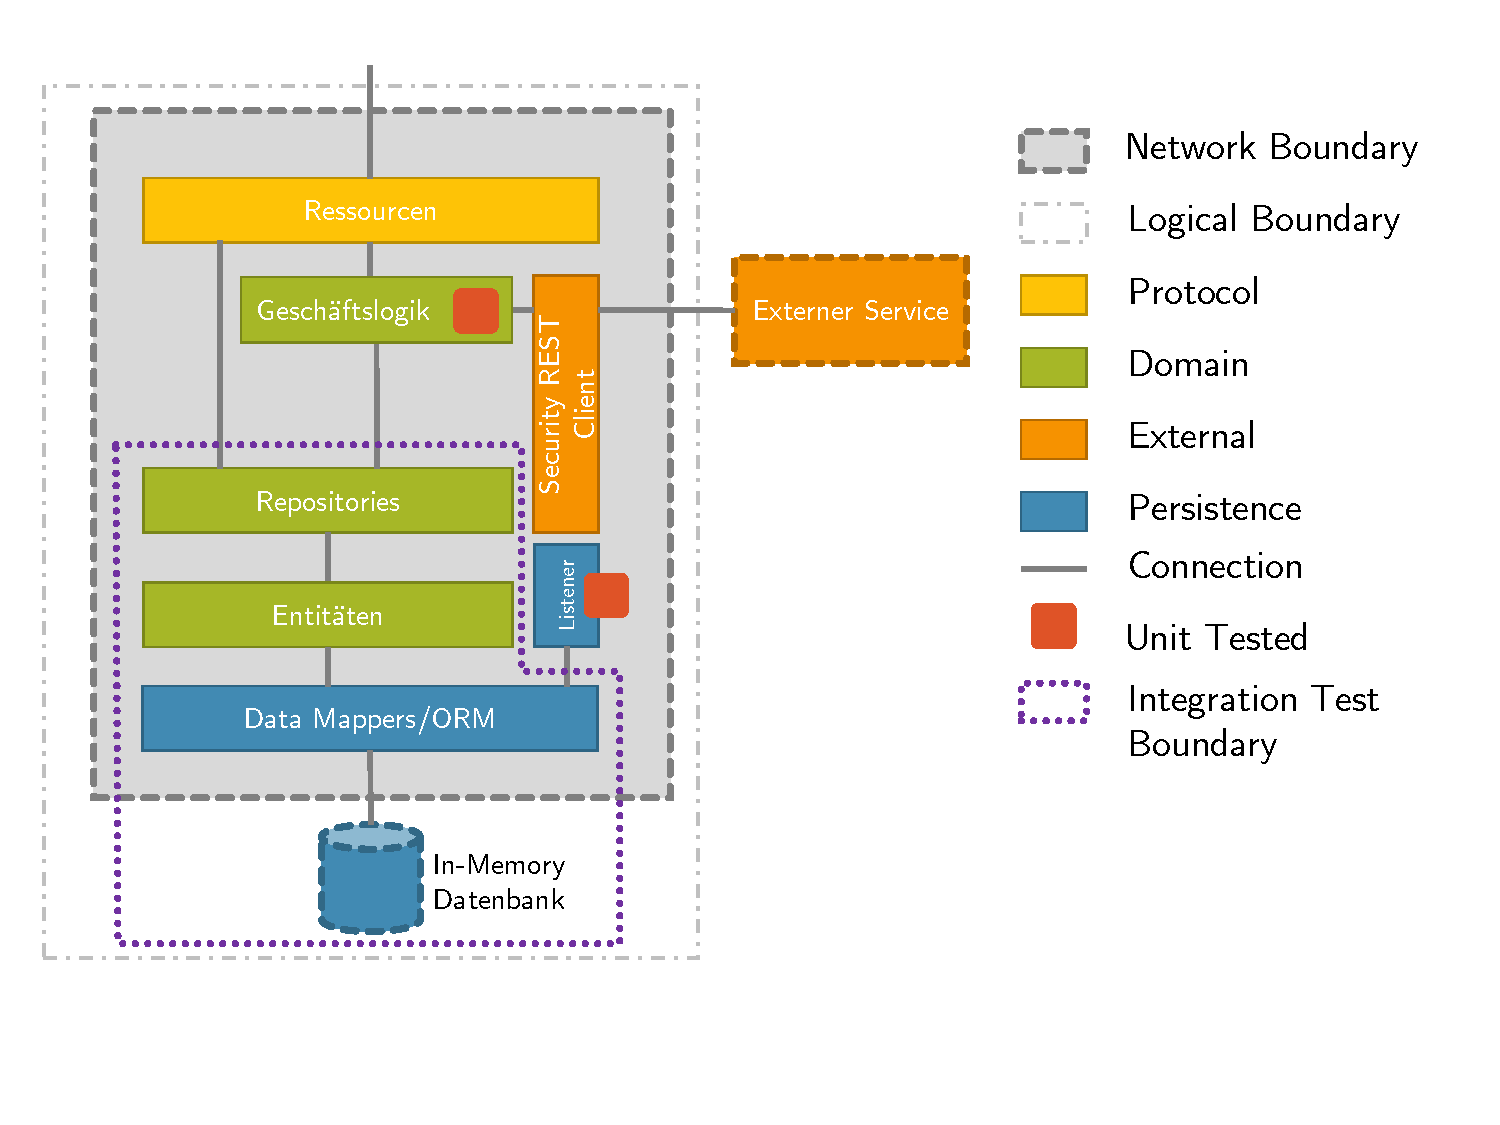
\includegraphics[width=0.9\linewidth]{images/img_integration-testing.pdf}
	\captionof{figure}[Integration Testing Scope]{Integration Testing Scope \cite{clemson}}
	\label{fig:img_integration-testing}
\end{minipage}
\end{comment}

\paragraph{Komponententests}

\begin{comment}
\vspace{1em}
\begin{minipage}{\linewidth}
	\centering
	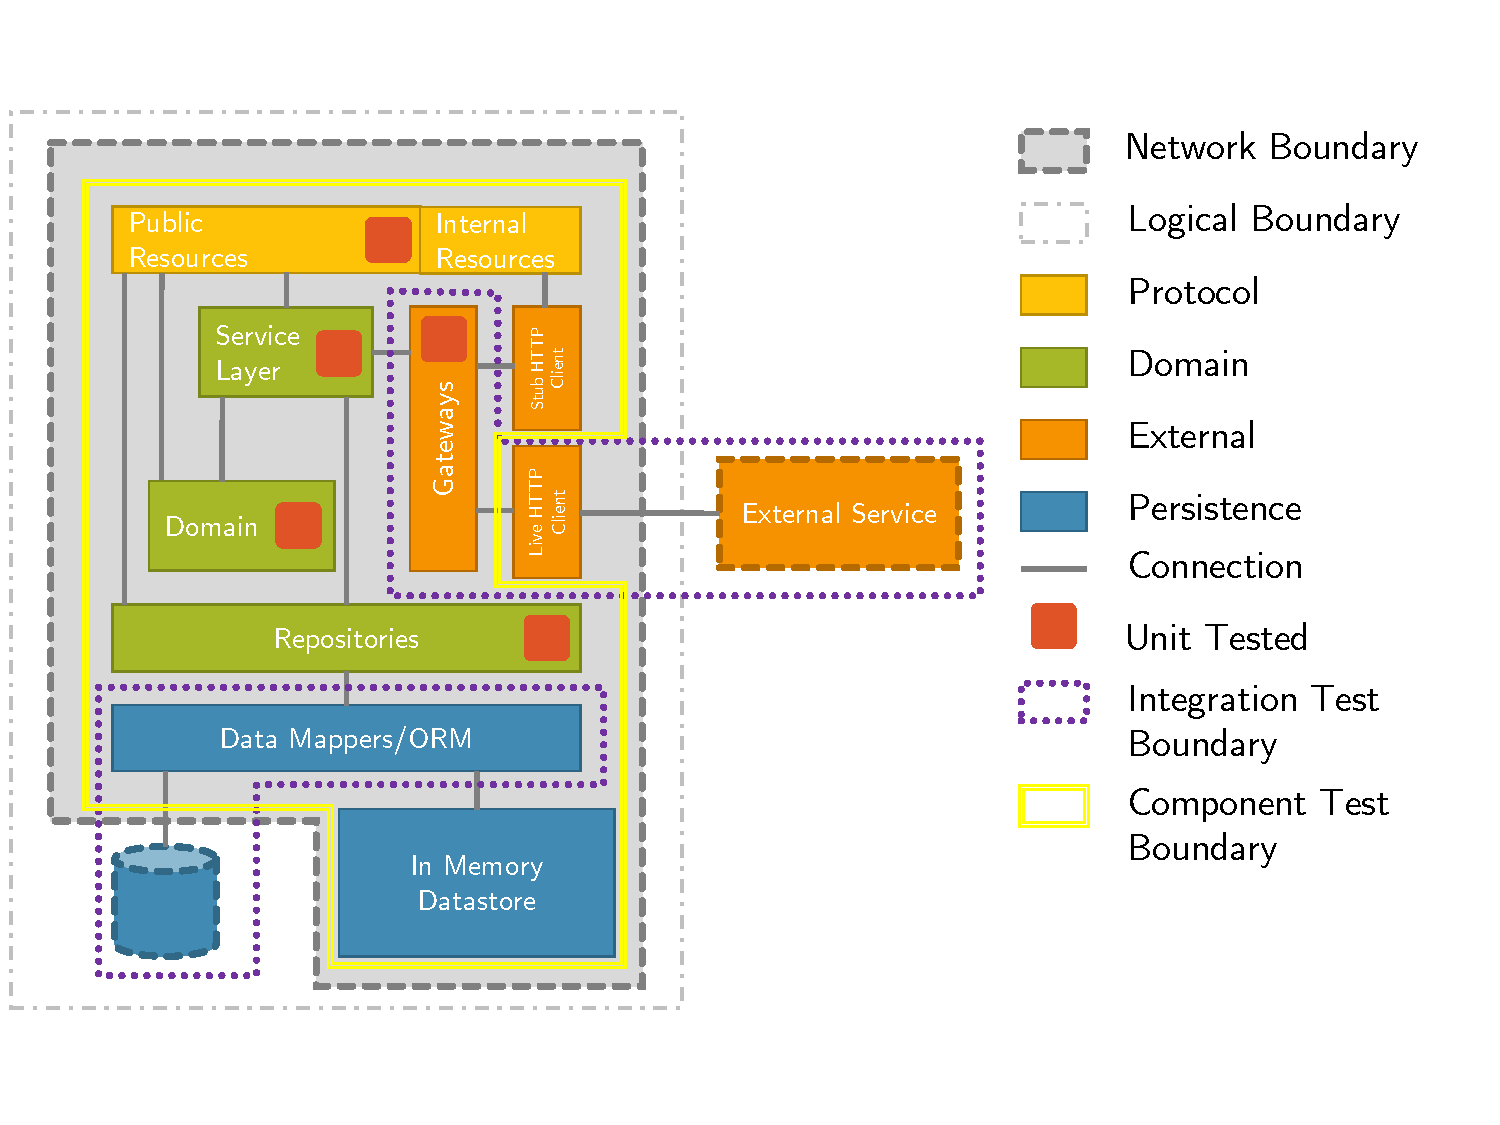
\includegraphics[width=0.9\linewidth]{images/img_component-testing.pdf}
	\captionof{figure}[Component Testing Scope]{Component Testing Scope \cite{clemson}}
	\label{fig:img_component-testing}
\end{minipage}
\end{comment}

\paragraph{Contract Testing}

\begin{comment}
\vspace{1em}
\begin{minipage}{\linewidth}
	\centering
	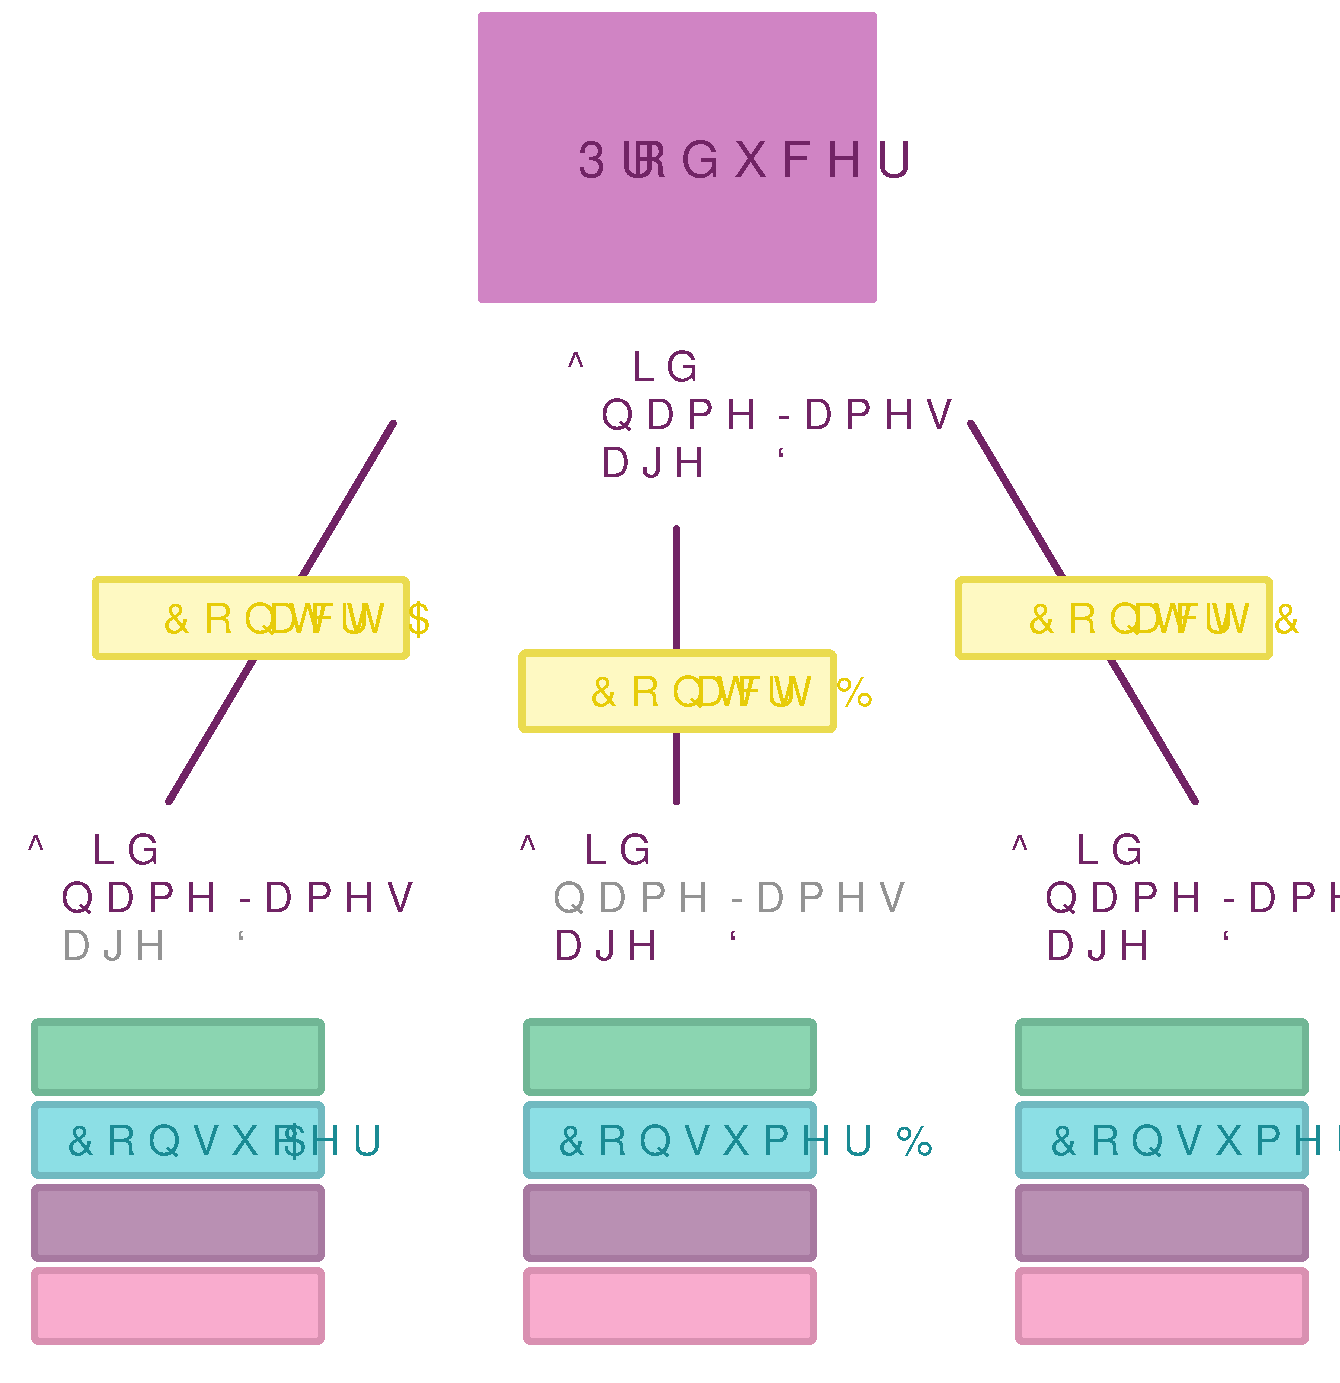
\includegraphics[width=0.9\linewidth]{images/img_contract-testing.pdf}
	\captionof{figure}[Contract Testing]{Contract Testing \cite{clemson}}
	\label{fig:img_contract-testing}
\end{minipage}
\end{comment}

\paragraph{End-To-End Testing}

\begin{comment}
\vspace{1em}
\begin{minipage}{\linewidth}
	\centering
	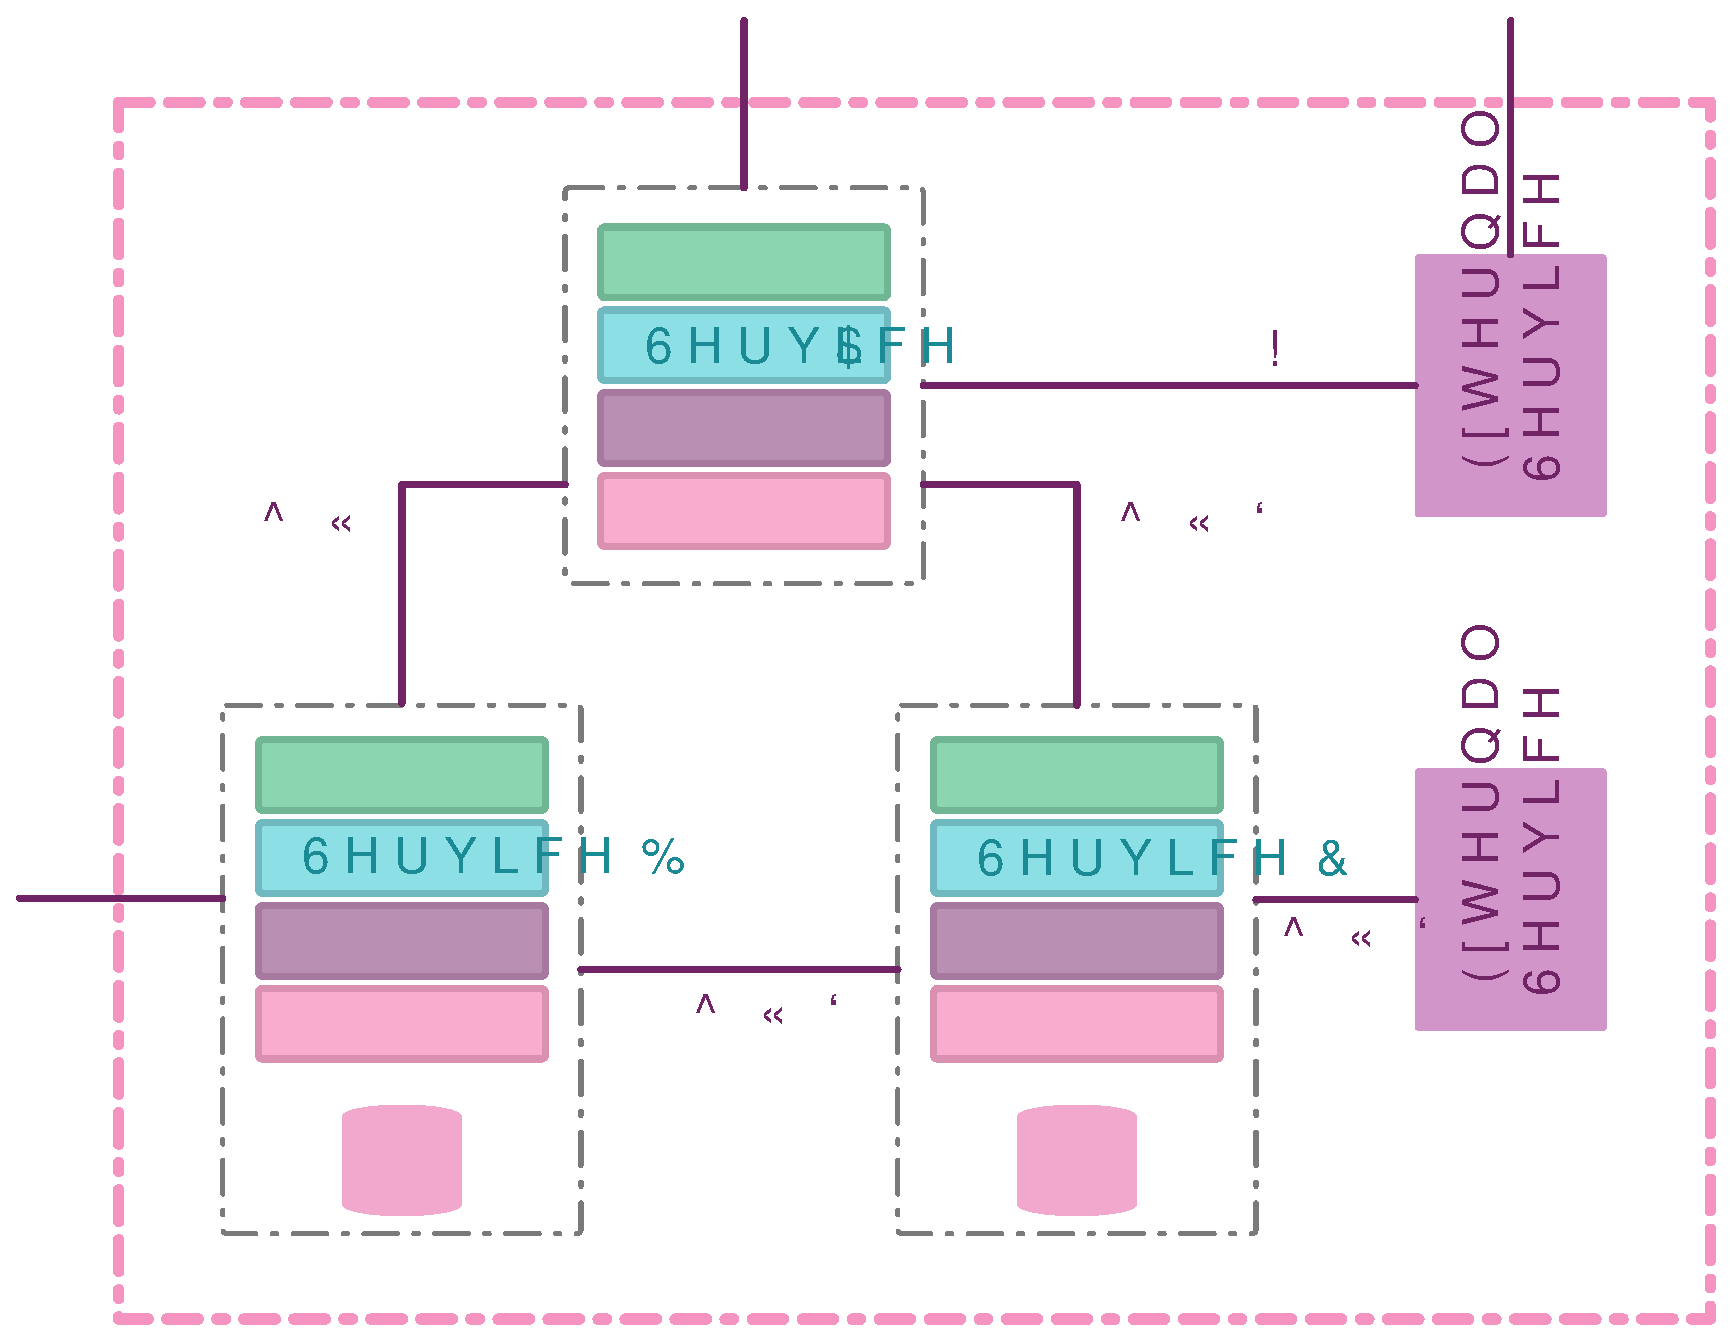
\includegraphics[width=0.9\linewidth]{images/img_end-to-end-testing.pdf}
	\captionof{figure}[End-To-End Testing Scope]{End-To-End Testing Scope \cite{clemson}}
	\label{fig:img_end-to-end-testing}
\end{minipage}
\end{comment}

\subsubsection{Sinnvolle Teststrategien für den generativen Ansatz}

\subsubsection{Frameworks zum Umsetzen von Test-Strategien}

% ----------------------------------------------------------------------------------------------------------
% Anforderungen an generierte Tests
% ----------------------------------------------------------------------------------------------------------
\section{Anforderungen an generierte Tests}

\subsection{Benötigte Daten}

\subsection{Notwendige Änderungen/Erweiterungen von Barrakuda}

% ----------------------------------------------------------------------------------------------------------
% Implementierung in Barrakuda
% ----------------------------------------------------------------------------------------------------------
\section{Implementierung in Barrakuda}

\subsection{Referenz-System}

\subsubsection{Komponenten und Aufbau}

\subsubsection{Implementierung des Systems}

\subsubsection{Implementierung der Tests}

\subsection{Übernahme der Referenz-Implementierung in Barrakuda-Templates}

% ----------------------------------------------------------------------------------------------------------
% Literatur
% ----------------------------------------------------------------------------------------------------------
\renewcommand\refname{Quellenverzeichnis}
\bibliographystyle{bibstyle}
\bibliography{bibfile}
\pagebreak

% ----------------------------------------------------------------------------------------------------------
% Anhang
% ----------------------------------------------------------------------------------------------------------
\pagenumbering{Roman}
\setcounter{page}{1}
\lhead{Anhang \thesection}

\begin{appendix}
\section*{Anhang}
\phantomsection
\addcontentsline{toc}{section}{Anhang}
\addtocontents{toc}{\vspace{-0.5em}}

\section{Code-Fragmente}
Viel Beispiel-Code

\end{appendix}

\end{document}
